\subsection{Lab19: Modulación QPSK en GRC}

%*********************
\begin{frame}{}

\pgfdeclareimage[width=\paperwidth,height=\paperheight]{bg}{imagenes/fondo_lab}
\setbeamertemplate{background}{\pgfuseimage{bg}}

\bfseries{\textrm{ \Large Lab 19: \\Modulación QPSK en GRC}}
\raggedright
\end{frame}
%********************

%--------------------------------------------------------------------------------------------
\begin{frame}{Modulación QPSK en GRC}

\pgfdeclareimage[width=\paperwidth,height=\paperheight]{bg}{imagenes/fondo3}
\setbeamertemplate{background}{\pgfuseimage{bg}}

\justifying
Este ejercicio mostrará la modulación digital QPSK en GRC donde los datos a enviar serán generados por el bloque Random Source el cual proveerá diferentes valores de manera aleatoria en el rango de 0 a 100, estos datos serán entregados en forma de bytes,para poderlos visualizar en un osciloscopio\cite{Universidad Militar Nueva Granada}

\end{frame}
%---------------------------------------------------------------------------
%\includegraphics[scale=1]{../imagenes/descarga.jpeg} 
\begin{frame}{Modulación QPSK en GRC}
\begin{figure}
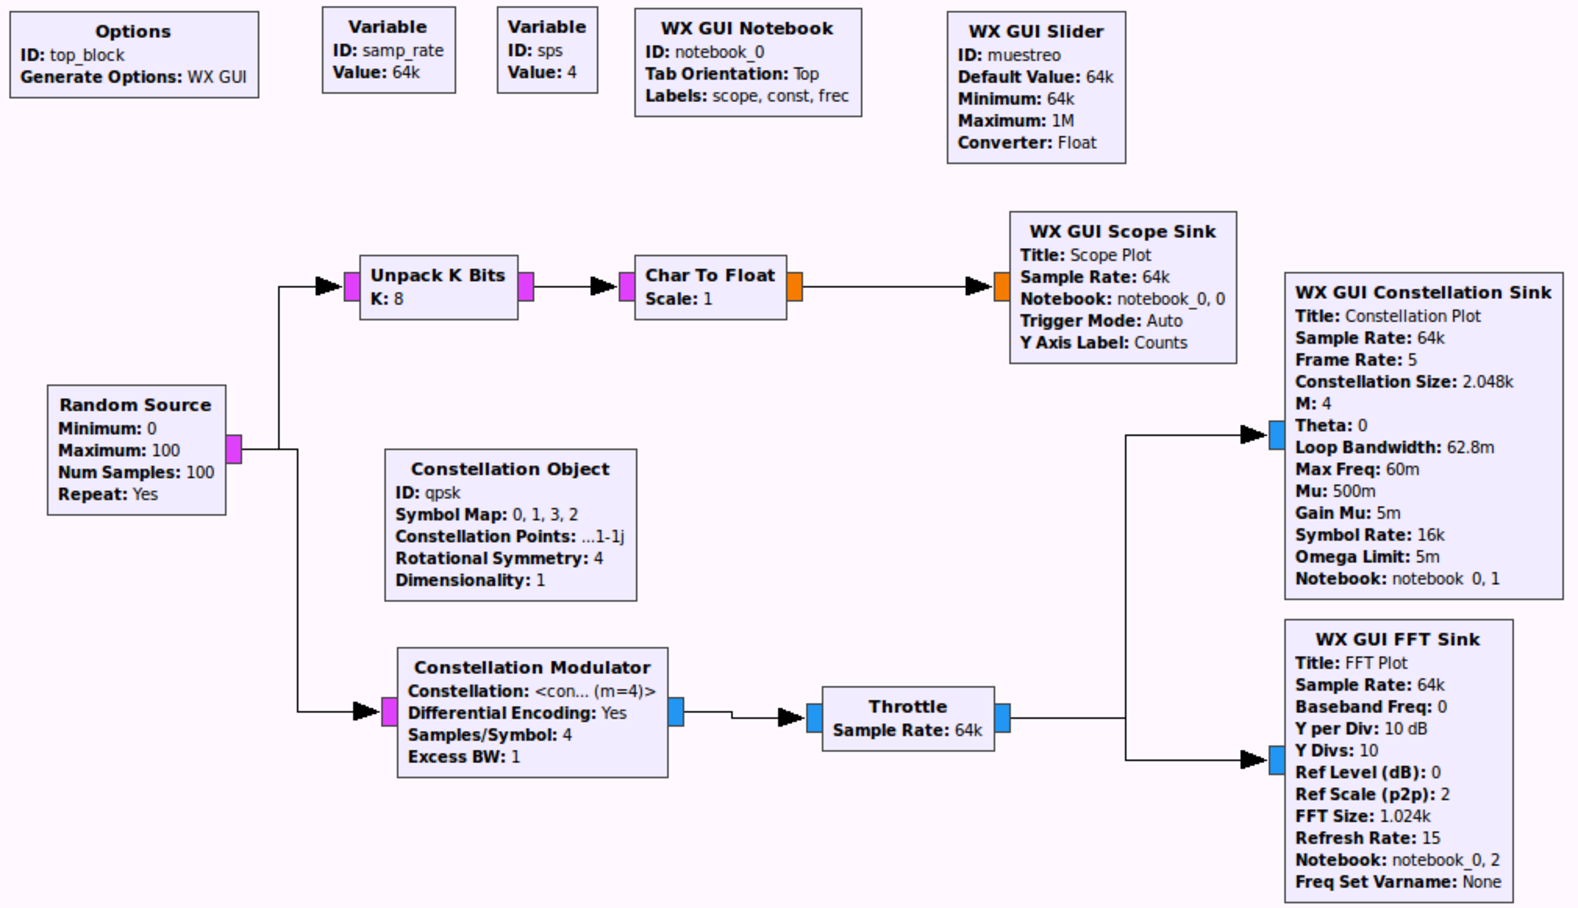
\includegraphics[scale=.4]{Modulaciones_digitales/lab19/pdf/lab19_1.pdf}
\end{figure}
\end{frame}
%--------------------------------------------------------------------------------------
\begin{frame}{Modulación QPSK en GRC}
\begin{figure}
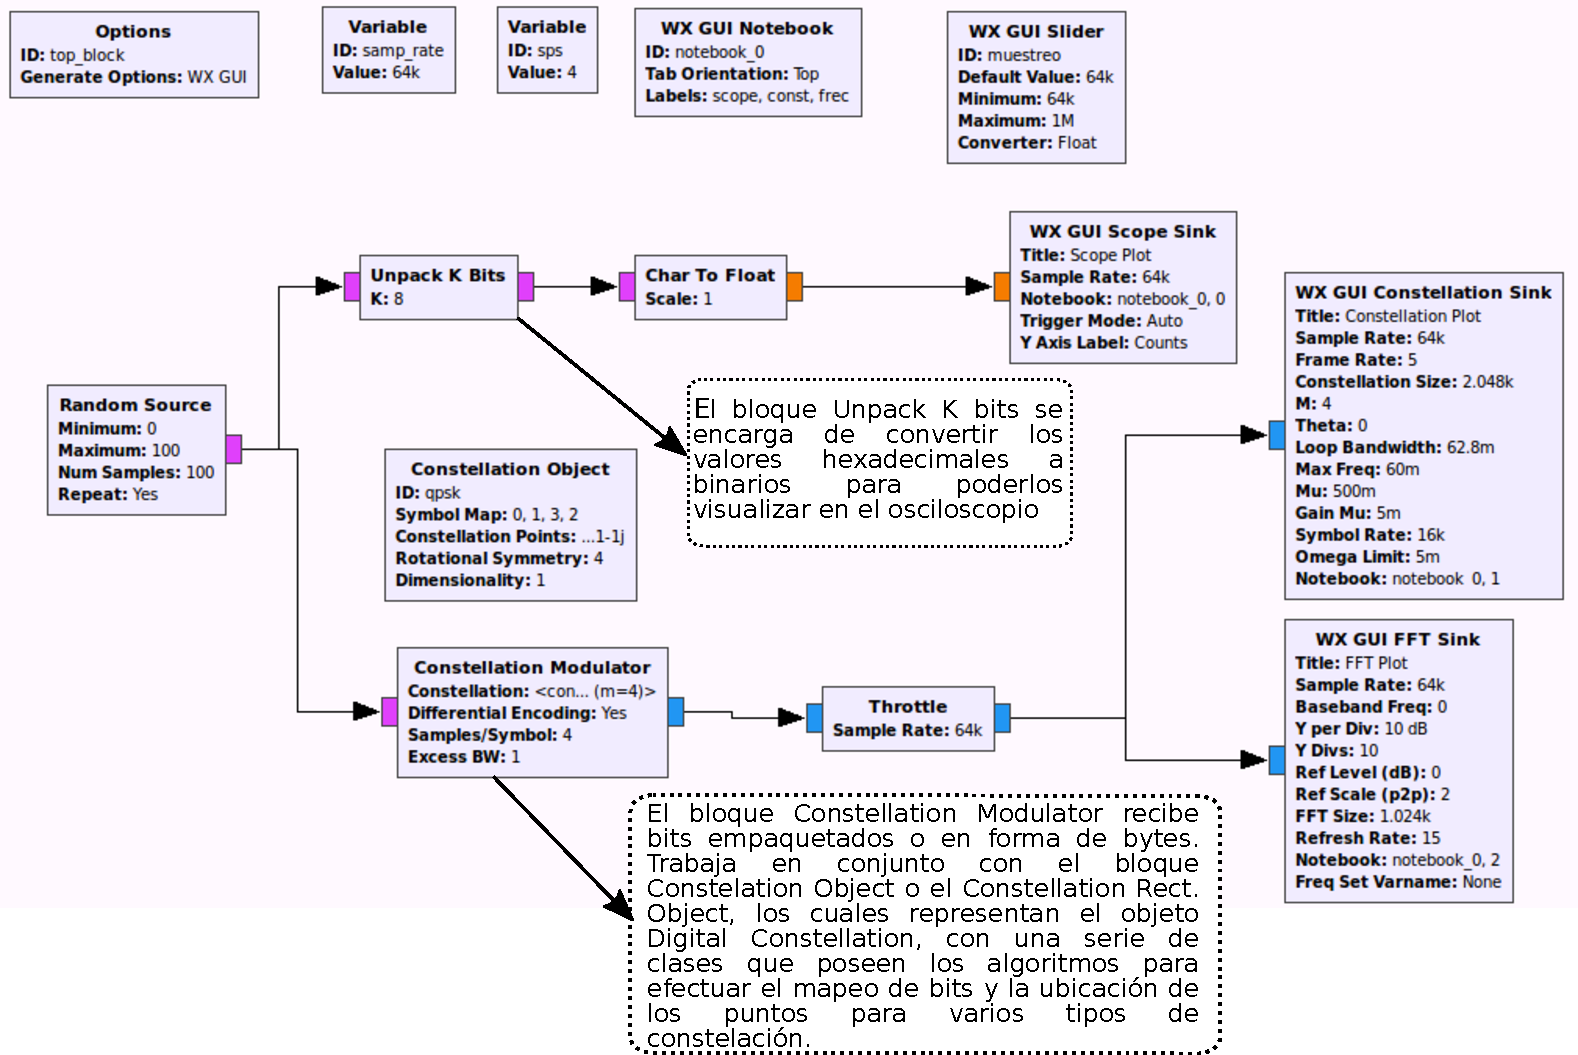
\includegraphics[scale=.35]{Modulaciones_digitales/lab19/pdf/lab19_2.pdf}
\end{figure}
\end{frame}
%-----------------------------------------------------------------------------------
\begin{frame}{Modulación QPSK en GRC}
Pulsos de señal generados por Random Source
\begin{figure}
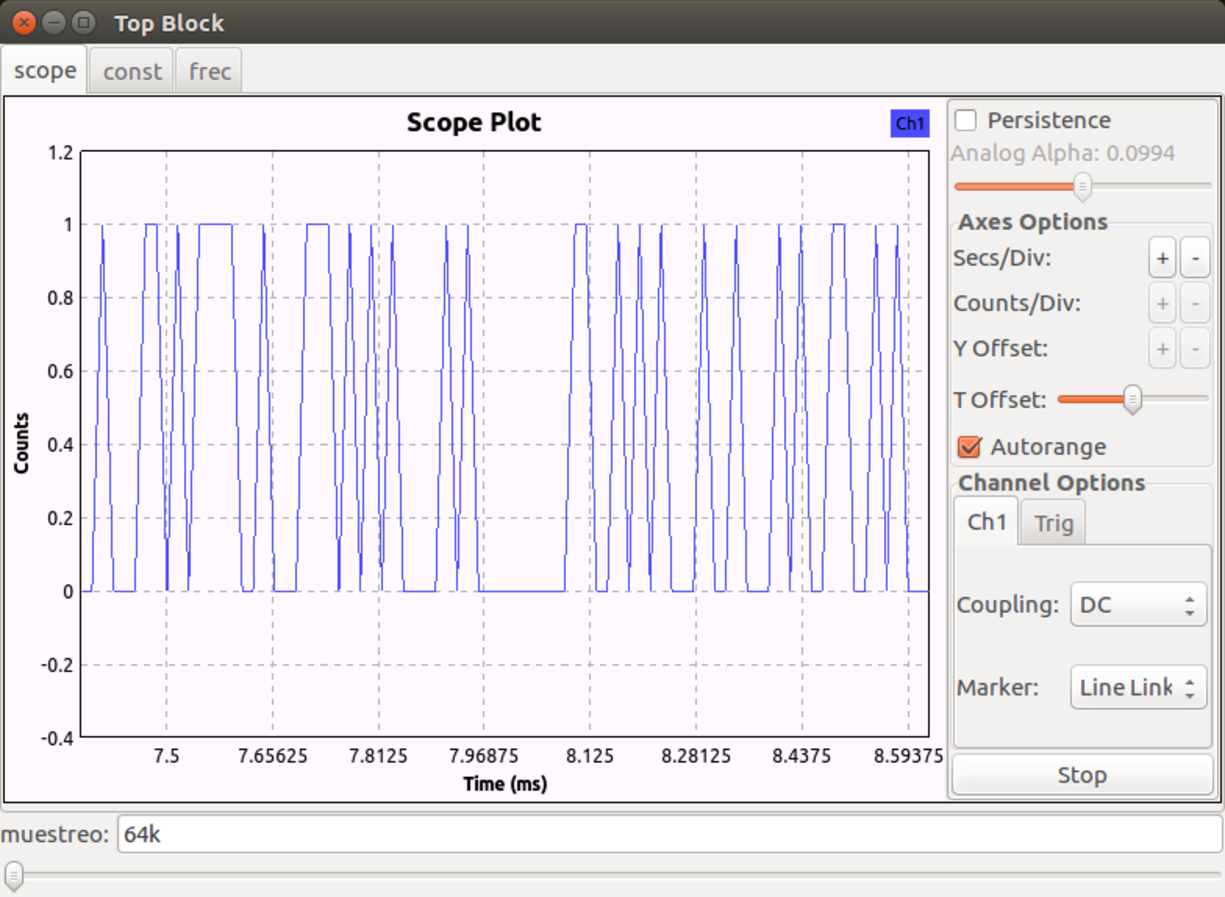
\includegraphics[scale=.4]{Modulaciones_digitales/lab19/pdf/lab19_3.pdf}
\end{figure}
\end{frame}
%---------------------------------------------------------------------------------------

\begin{frame}{Modulación QPSK en GRC}
\justifying
La definición de la constelación en el bloque Constellation Object se efectua de acuerdo a la cantidad de símbolos posibles en la misma dentro del espacio complejo o el diagrama de constelación. Para la constelación de QPSK se manejan 4 símbolos, entonces de acuerdo a la siguiente ecuación los bits para cada símbolo serían 2.\\
\centering
$\log_{2}(4)=2$ bits/símbolo\\
\end{frame}

%--------------------------------------------------------------------------------

\begin{frame}{Modulación QPSK en GRC}
\begin{figure}
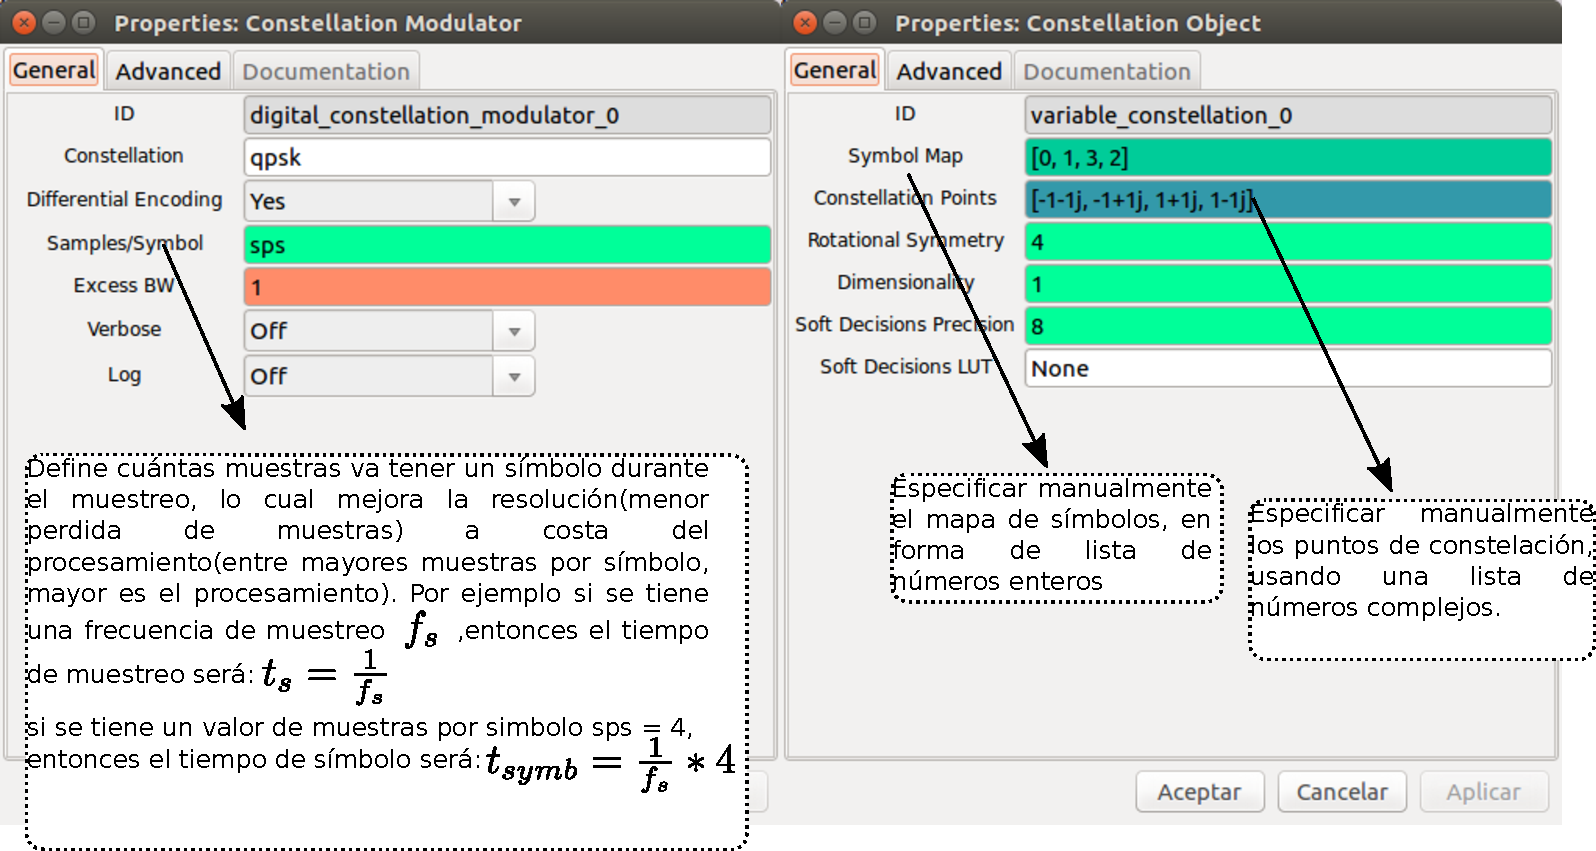
\includegraphics[scale=.4]{Modulaciones_digitales/lab19/pdf/lab19_4.pdf}
\end{figure}
\end{frame}
%-----------------------------------------------------------------------------------

%---------------------------------------------------------------------------------------
\begin{frame}{Modulación QPSK en GRC}
\justifying
En el bloque Constellation modulator es posible implementar codificación diferencial con tan sólo habilitar este parámetro dentro de la configuración. La codificación diferencial o modulación diferencial en fase, no siempre asigna una fase determinada a cada símbolo (0 o 1), sino que de acuerdo a cada transición de bit, el modulador efectúa un cambio de fase de la siguiente manera:\\
\begin{itemize}
\item Si el siguiente símbolo es un 1 el cambio de fase es de $270^{\circ}$  
\item Si el siguiente símbolo es un 1 el cambio de fase es de $90^{\circ}$
\end{itemize}
La codificación diferencial contribuye a la reducción de errores y hace la modulación QPSK más robusta frente a la sensibilidad de ruido debido a los saltos de fase, puesto que no es necesario una demodulación síncrona con la portadora.\cite{Universidad Militar Nueva Granada}
\end{frame}

%---------------------------------------------------------------------------
\begin{frame}{Modulación QPSK en GRC}
\justifying
Constelación QPSK con codificación diferencial habilitada y 4 Muestras por símbolo
\begin{figure}
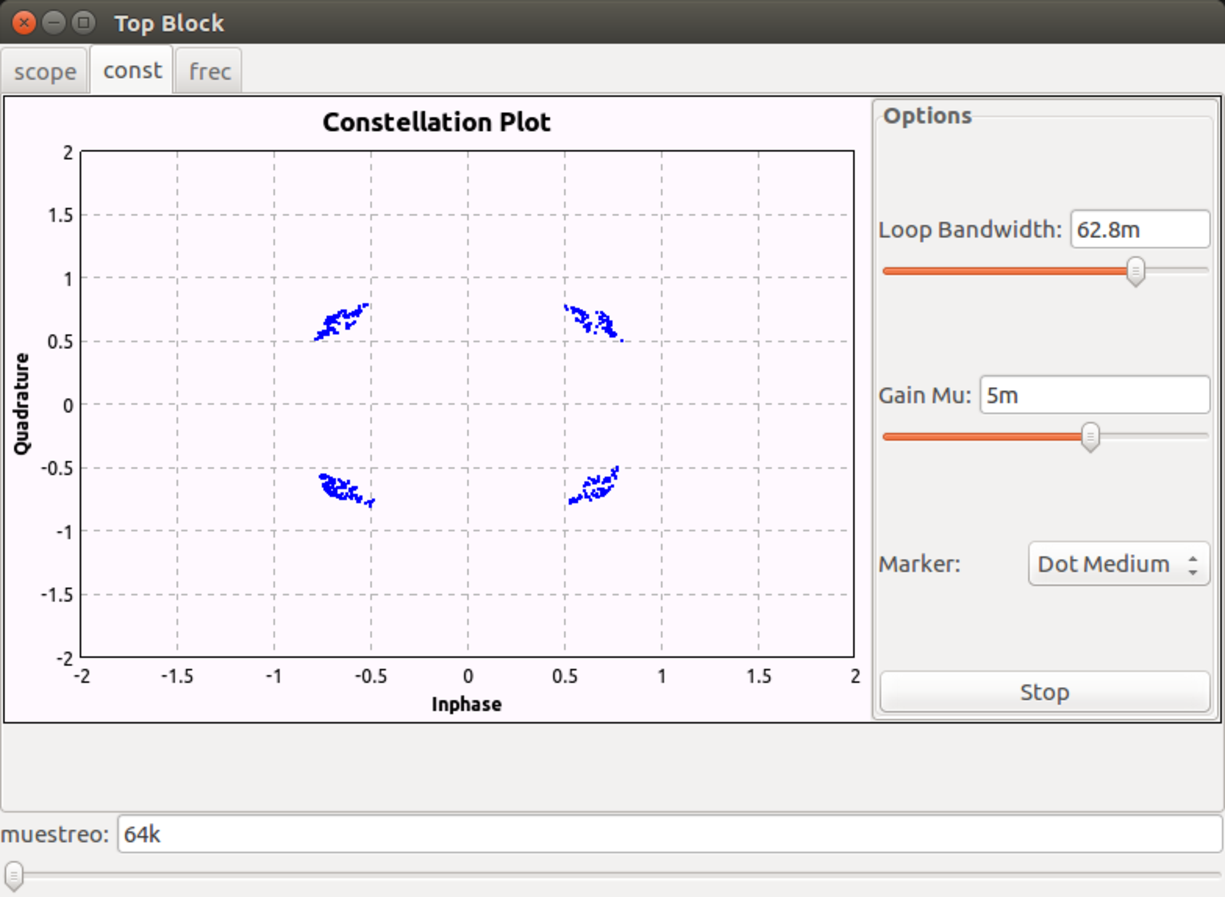
\includegraphics[scale=.4]{Modulaciones_digitales/lab19/pdf/lab19_5.pdf}
\end{figure}
\end{frame}
%-------------------------------------------------------------------------------------------
%\begin{frame}{Modulación QPSK en GRC}
%\begin{figure}
%\includegraphics[width=.9\textwidth]{parte1/QPSK/pdf/QPSK_6.pdf}
%\end{figure}
%\end{frame}
%------------------------------------------------------------------------------------------
\begin{frame}{Modulación QPSK en GRC}
Espectro de señal QPSK modulada a una frecuencia de muestreo igual a 64 kHz
\begin{figure}
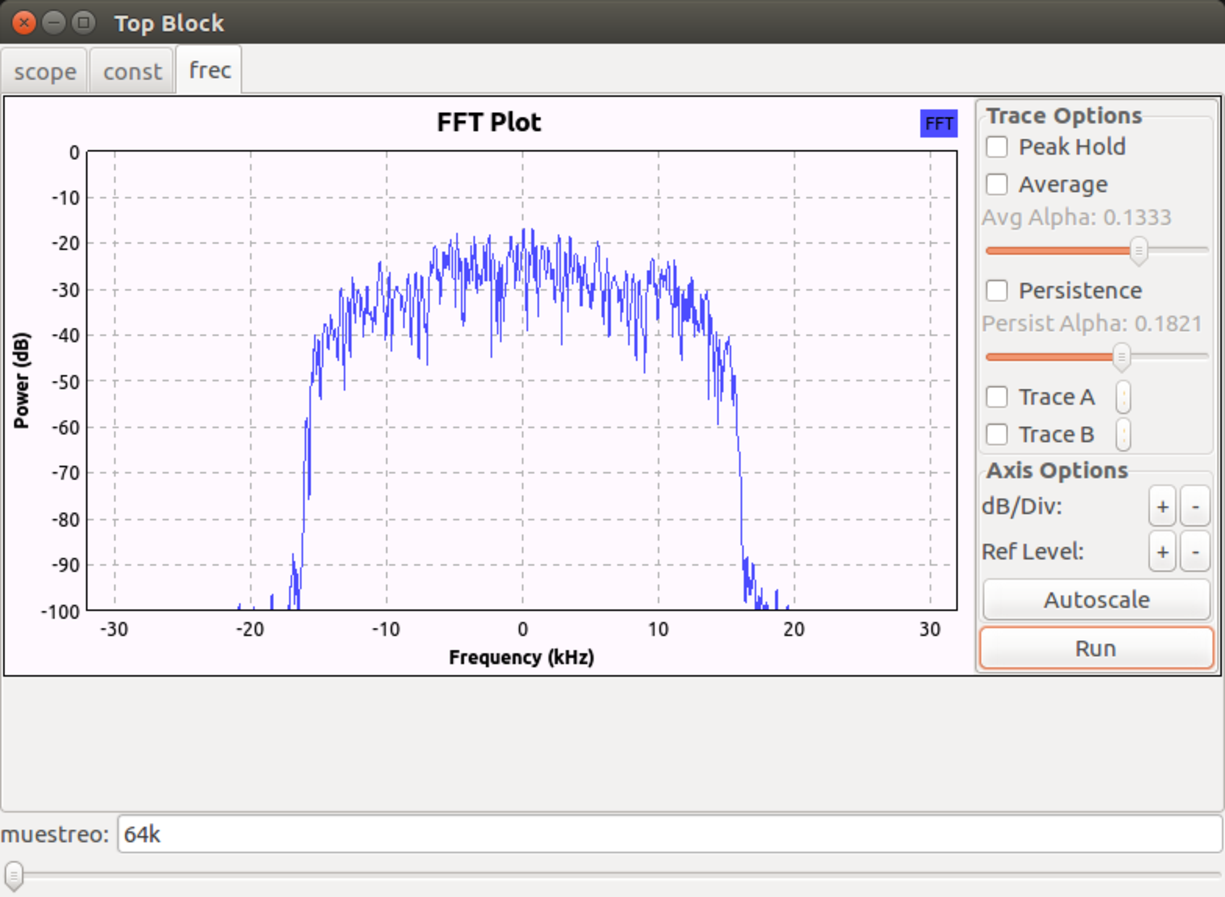
\includegraphics[width=.8\textwidth]{Modulaciones_digitales/lab19/pdf/lab19_7.pdf}
\end{figure}
\end{frame}
